\documentclass[bachelor]{iisthesis}
%           or master (bachelor or master is required)

% These two packages are highly recommended:
\usepackage[T1]{fontenc} % make non-ASCII characters cut&pastable in PDF
\usepackage{lmodern}     % easiest way to get outline fonts with T1 encoding

% \usepackage[ngerman]{babel}     % if the thesis is written in German

\title{IIS Thesis Instructions}
\author{Stephen Cobeldick}
\supervisor{Justus Piater}
%\supervisor{Firstname1 Lastname1\\ Firstname2 Lastname2}


\begin{document}
\maketitle

\chapternn{Abstract}
This document explains how to write IIS theses using the \LaTeXe\space `\uibkclass' class\footnote{version \uibkversion\space, released on \uibkreleased.}, which is itself based on the \LaTeXe\space `book' class and is intended for compiling with pdflatex. This document does not tell you how to structure your thesis.

\chapternn{Acknowledgments}
Thank you to the friendly members of the IIS Team.

\tableofcontents
\listoffigures
\listoftables
\uibkdeclaration
\label{chap:declare}

\chapter{Introduction}
Your thesis should begin with an introduction, background information and descriptions of existing works. For example the `\uibkclass' class package dependencies could be considered to be background information, and are shown in \autoref{tab:depend}. For an excellent introduction to writing a thesis using \LaTeX\space you should read \cite{Talbot-2007-ThesisGuide}'s exceptionally good guide, which is available both online and as a PDF.

\begin{table}
  \centering
  \begin{tabular}{|l|l|}
    \hline
    Package:            & Function: \\
    \hline
    \texttt{xcolor}   & Text + hyperlink colors    \\
    \texttt{natbib}   & Bibliography style         \\
    \texttt{anysize}  & Margins                    \\
    \texttt{graphicx} & Insert logo image          \\
    \texttt{hyperref} & Hyperlinks                 \\
    \texttt{hypcap}   & Hyperlinks to top of floats\\
    \hline
  \end{tabular}
  \caption{Package Dependencies}
  \label{tab:depend}
\end{table}

\chapter{Technical Content}
This is the bulk of your thesis, several chapters with lots of nice illustrations, e.g.\ \autoref{fig:dog}.  It is good style to cite people, not publications, as recommends \cite{Piater-2011-IISreport}.  Web references should be avoided to the extent possible because they cannot usually be considered \emph{archival} \citep{Wikipedia-Archive}, and require careful assessment of reliability.

\begin{figure}[h]
  \centering
  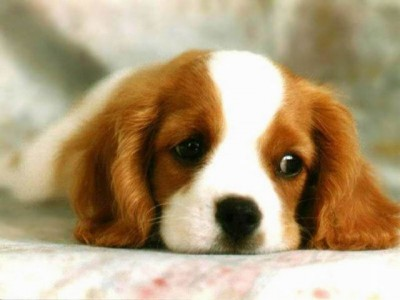
\includegraphics[width=0.6\textwidth]{dog.jpg}
  \caption{Cute Dog}
  \label{fig:dog}
\end{figure}

\section{Multiple \texttt{.tex} Files}
\texttt{\textbackslash include\{file\_name\}} and \texttt{\textbackslash includeonly\{\ldots\}} lets you write your thesis chapters in multiple \texttt{.tex} files and then join these into one document. This is also an excellent way to manage compilation of large documents, especially to help locate the source of any error messages and allow easy rearrangement of your thesis chapters and sections.

\section{Single / Double Sided Pages}
\begin{tabular}{|l|l|l|}
  \hline
  Class Option:              & Intended For:           & Hyperlinks: \\
  \hline
  \texttt{oneside}           & electronic (PDF) copies & colorlinks  \\
  \texttt{twoside} (default) & printing and binding.   & colorborders\\
  \hline
\end{tabular}

\section{UIBK Colors}
The `\uibkclass' class uses the official UIBK colors for citations and hyperlinks within the document. To maintain a thematic consistency, you can use these colors in your own diagrams and images: \textcolor{uibkorange}{\texttt{uibkorange}} and \textcolor{uibkblue}{\texttt{uibkblue}}.

\chapter{Special Commands}
The `\uibkclass' class provides some convenient commands to help you write your thesis.

\section{\textbackslash logoimage}
\texttt{\textbackslash logoimage}\\
\texttt{\textbackslash logoimage[file\_name]}\\[\baselineskip]
By default the `\uibkclass' class will look for a UIBK logo file named ``{Uni\_Logo\_4C.eps}'': this UIBK \texttt{.eps} logo has the best print quality (and if compiling with pdflatex you will need to use the package `epstopdf'). If you wish to use another logo image, then this command lets you select a specific file. If momentarily you do not have access to a UIBK logo file, simply call this command with no argument.

\section{\textbackslash title}
\label{sec:title}
\texttt{\textbackslash title\{one\_line\}}\\
\texttt{\textbackslash title[first\_line]\{second\_line\}}\\[\baselineskip]
This command has been altered to provide an optional input if you wish your title to appear over two lines on the titlepage, with the correct spacing.

\section{\textbackslash maketitle}
\texttt{\textbackslash maketitle}\\[\baselineskip]
This command creates the titlepage by placing the UIBK logo in the top left and placing the university, institute and group names together with the thesis \hyperref[sec:title]{title}, author and date along the right margin. The command also sets the page margins, pagestyle and page numbering for the title page, and for the rest of the front matter.

\section{\textbackslash chapternn}
\texttt{\textbackslash chapternn\{full\_name\}}\\
\texttt{\textbackslash chapternn[toc\_name]\{full\_name\}}\\[\baselineskip]
No-number chapters, improving the standard \LaTeX\space command \texttt{\textbackslash chapter*} by also including the chapter name in the headers, bookmarks and table of contents.

\section{\textbackslash uibkdeclaration}
\texttt{\textbackslash uibkdeclaration}\\[\baselineskip]
Inserts a new chapter with the UIBK author's \hyperref[chap:declare]{declaration}. Signature and date fields are indicated below the declaration. This command must appear last in your front matter (i.e.\ immediately before the first chapter) as it also sets the pagestyle and page numbering for the thesis' main matter.

\chapter{Conclusions}
Your thesis should conclude with a summary of the highlights, any conclusions to be drawn, and descriptions of possible future work. And before you print your thesis, remember to use a spell-checker!

\bibliography{refs}% Remember to compile the bibliography using bibtex.

\appendix% Start your appendices with this command.

\chapter{Proof}
Cubum autem in duos cubos, aut quadratoquadratum in duos quadratoquadratos, et generaliter nullam in infinitum ultra quadratum potestatem in duos eiusdem nominis fas est dividere cuius rei demonstrationem mirabilem sane detexi. Hanc marginis exiguitas non caperet\ldots

\chapter{Algebra}
L'alg\`ebre n'est qu'une g\'eom\'etrie \'ecrite; la g\'eom\'etrie n'est qu'une alg\`ebre figur\'ee.

\hfill Sophie Germain

\end{document}
